% Definir el documento
\documentclass[12pt]{report}
%%%%%%%%%%%%%%%%%%%%%%%%%%%%%%%
% Bibliotecas en el documento

\usepackage[spanish]{babel}
\usepackage[top=20mm, bottom=15mm, right=20mm, left=25mm]{geometry}
\usepackage{lipsum}

\usepackage{graphicx}
\usepackage{subcaption}
%%%%%%%%%%%%%%%%%%%%%%%%%%%%%%%

%%%%%%%%%%%%%%%%%%%%%%%%%%%%%%%
% Configuración del documento

\graphicspath{{./figures}}
\setlength{\parindent}{0pt}
\setlength{\parskip}{12pt}
%%%%%%%%%%%%%%%%%%%%%%%%%%%%%%%

%%%%%%%%%%%%%%%%%%%%%%%%%%%%%%%
% Datos del documento

\title{Introducción a \LaTeX}
\date{\today}
\author{Yo mismo}

%%%%%%%%%%%%%%%%%%%%%%%%%%%%%%%

\begin{document}

	\maketitle
	\tableofcontents
	
	%Definir un capítulo nuevo
	\chapter{Mi primer capítulo}
		
		En la figura \ref{fig:latex-logo}
		\lipsum[1][1-11]
	
		\begin{figure}[h]
			\centering
			\begin{subfigure}{0.4\textwidth}
				\centering
				
\includegraphics[
					width=\linewidth,
					height=40mm,
					keepaspectratio
				]{latex.png}
				\caption{Logo de \LaTeX}
				\label{fig:latex-logo}
			\end{subfigure}
			\hfill
			\begin{subfigure}{0.4\textwidth}
				\centering
				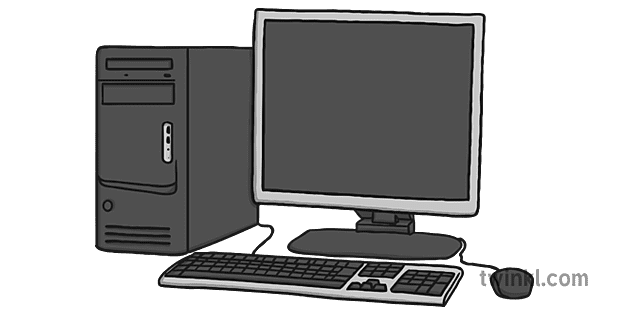
\includegraphics[
					width=\linewidth,
					height=40mm,
					keepaspectratio
				]{computer.png}
				\caption{Imagen de computadora}
				\label{fig:computer-image}
			\end{subfigure}
			\caption{Figura grande}
			\label{fig:grande}
		\end{figure}
		
		Hola \hfill mundo
		
		\section{Mi primer sección}
			\lipsum[1-2]
			\lipsum[1][1-3]
		
		% Definir una sección nueva
		\section{Mi segunda sección}
			\lipsum[3-5]
% Termina nuestro documento
\end{document}